%%p01
Hallar el cociente de:
\begin{figure}[h]
	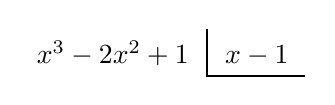
\begin{tikzpicture}[thick]
		\node[above left] at (-.1,0) {$x^3-2x^2+1$};
		\node[above right] at (.1,0) {$x-1$};
		\draw (0,.6) -- (0,0) -- (1.25,0);
	\end{tikzpicture}
\end{figure}
%%a01
\begin{enum}
	* $x^2-x-1$
	* $x^5-2x-5$
	* $x^4-x-1$
	* $x^9-x-1$
\end{enum}
%%r01
$x^2-x-1$
%%p02
Hallar el cociente de:
\begin{figure}[h]
	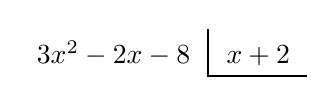
\begin{tikzpicture}[thick]
		\node[above left] at (-.1,0) {$3x^2-2x-8$};
		\node[above right] at (.1,.0) {$x+2$};
		\draw (0,.6) -- (0,0) -- (1.25,0);
	\end{tikzpicture}
\end{figure}
%%a02
\begin{enum}
	* $2x-8$
	* $2x-6$
	* $4x+9$
	* $3x-8$
\end{enum}
%%r02
$3x-8$
%%p03
Hallar el cociente de: \\
$4x^3+2x-x$ entre $3-x^2$.
%%a03
\begin{enum}
	* $x^2$
	* $-4x$
	* $4x$
	* $3x$
\end{enum}
%%r03
$-4x$
%%p04
Hallar el cociente de:
\begin{figure}[h]
	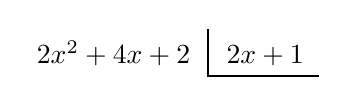
\begin{tikzpicture}[thick]
		\node[above left] at (-.1,0) {$2x^2+4x+2$};
		\node[above right] at (.1,0) {$2x+1$};
		\draw (0,.6) -- (0,0) -- (1.4,0);
	\end{tikzpicture}
\end{figure}
%%a04
\begin{enum}
	* $x+\dfrac{2}{3}$
	* $x-\dfrac{3}{2}$
	* $x-\dfrac{2}{3}$
	* $x+\dfrac{3}{2}$
\end{enum}
%%r04
$x+\dfrac{3}{2}$
%%p05
$(2x+1)\cdot\left(1+x-x^2\right)$
%%a05
\begin{enum}
	* $2x^3-x^2+3x+1$
	* $2x^3+x^2-2x+2$
	* $-2x^3+x^2+3x+1$
	* $-2x^2-x^3-3x+1$
\end{enum}
%%r05
$-2x^3+x^2+3x+1$
%%p06
$\left(2+3x+x^2\right)\cdot(2+x)$
%%a06
\begin{enum}
	* $6-10x+2x^2-x^3$
	* $5-7x+3x^2-6$
	* $4+8x+5x^2+x^3$
	* $7+8x^2+10x^3$
\end{enum}
%%r06
$4+8x+5x^2+x^3$
%%p07
$\left(4x^2+3x\right)\cdot\left(x^3-5x^2+2x\right)$
%%a07
\begin{enum}
	* $4x^5-17x^4-7x^3+6x^2$
	* $-14x^3-18x+12-16$
	* $8$
	* $7$
\end{enum}
%%r07
$4x^5-17x^4-7x^3+6x^2$
%%p08
Hallar el cociente de:
\begin{figure}[h]
	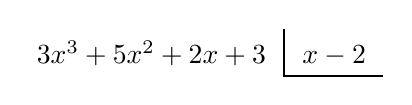
\begin{tikzpicture}[thick]
		\node[above left] at (-.1,0) {$3x^3+5x^2+2x+3$};
		\node[above right] at (.1,0) {$x-2$};
		\draw (0,.6) -- (0,0) -- (1.25,0);
	\end{tikzpicture}
\end{figure}
%%a08
\begin{enum}
	* $3x^2+24-11x$
	* $2x+13-24x^2$
	* $3x^2+11x-24$
	* $3x^2+11x+24$
\end{enum}
%%r08
$3x^2+11x+24$
%%p09
Hallar el cociente de:
\begin{figure}[h]
	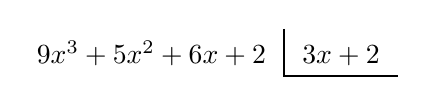
\begin{tikzpicture}[thick]
		\node[above left] at (-.1,0) {$9x^3+5x^2+6x+2$};
		\node[above right] at (.1,0) {$3x+2$};
		\draw (0,.6) -- (0,0) -- (1.45,0);
	\end{tikzpicture}
\end{figure}
%%a09
\begin{enum}
	* $3x^2-\dfrac{1}{3}x+\dfrac{20}{9}$
	* $2x^3-\dfrac{1}{4}x+\dfrac{20}{7}$
	* $7x^{11}-\dfrac{1}{9}x+\dfrac{22}{8}$
	* $9x^2-\dfrac{1}{6}x+\dfrac{11}{4}$
\end{enum}
%%r09
$3x^2-\dfrac{1}{3}x+\dfrac{20}{9}$
%%p10
Hallar el cociente de:
\begin{figure}[h]
	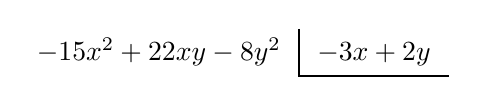
\begin{tikzpicture}[thick]
		\node[above left] at (-.1,0) {$-15x^2+22xy-8y^2$};
		\node[above right] at (.1,0) {$-3x+2y$};
		\draw (0,.6) -- (0,0) -- (1.9,0);
	\end{tikzpicture}
\end{figure}
%%a10
\begin{enum}
	* $5x-2y$
	* $3x+4y$
	* $5x-4y$
	* $7x-y$
\end{enum}
%%r10
$5x-4y$
%%p11
Hallar el cociente de: \\
$2x^4-x^3+x^2+7x-3$ entre $2x+3$.
%%a11
\begin{enum}
	* $x^3-2x^2+\dfrac{7}{2}x-\dfrac{7}{4}$
	* $x^5-9x^5+\dfrac{7}{2}x-\dfrac{7}{10}$
	* $x^6-2x^2+\dfac{7}{2}x-2$
	* $x^9-4x^3+\dfrac{1}{2}x-\dfrac{5}{3}$
\end{enum}
%%r11
$x^3-2x^2+\dfrac{7}{2}x-\dfrac{7}{4}$
%%p12
Hallar el cociente de:
\begin{figure}[h]
	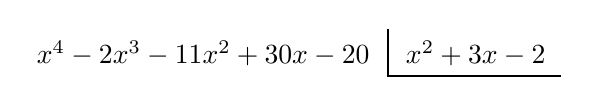
\begin{tikzpicture}[thick]
		\node[above left] at (-.1,0) {$x^4-2x^3-11x^2+30x-20$};
		\node[above right] at (.1,0) {$x^2+3x-2$};
		\draw (0,.6) -- (0,0) -- (2.2,0);
	\end{tikzpicture}
\end{figure}
%%a12
\begin{enum}
	* $x+5x^2$
	* $x^2-3x$
	* $2x-5x^2$
	* $x^2-5x+6$
\end{enum}
%%r12
$x^2-5x+6$
%%p13
Hallar el cociente de: \\
$6x^3-2x^2-15x+8$ entre $2x^2+x-5$.
%%a13
\begin{enum}
	* $3x-\dfrac{4}{2}$
	* $3x+\dfrac{10}{4}$
	* $3x+\dfrac{5}{7}$
	* $3x-\dfrac{5}{2}$
\end{enum}
%%r13
$3x-\dfrac{5}{2}$
%%p14
Hallar el cociente de:
\begin{figure}[h]
	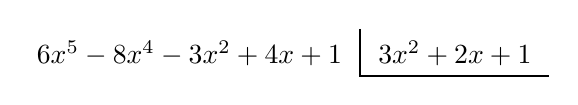
\begin{tikzpicture}[thick]
		\node[above left] at (-.1,0) {$6x^5-8x^4-3x^2+4x+1$};
		\node[above right] at (.1,0) {$3x^2+2x+1$};
		\draw (0,.6) -- (0,0) -- (2.4,0);
	\end{tikzpicture}
\end{figure}
%%a14
\begin{enum}
	* $3x^2+5x^2-2x+3$
	* $2x^3-4x^2+2x-1$
	* $3x^3-5x^2+2x-3$
	* $2x^2+4x^2-2x+1$
\end{enum}
%%r14
$2x^3-4x^2+2x-1$
%%p15
$\dfrac{6x^5-5x^3-35x-14x^2+23x^4+20}{3x^3-5+x^2}$
%%a15
\begin{enum}
	* $2x^2+7x-4$
	* $3x^2-8x+3$
	* $5x^4-7x+3$
	* $2x^2-7x+4$
\end{enum}
%%r15
$2x^2+7x-4$
